\documentclass[11pt]{article}
\usepackage[margin=1in]{geometry}
\usepackage{booktabs}
\usepackage{graphicx}
\usepackage{amsmath}
\usepackage{caption}
\usepackage[hidelinks]{hyperref}
\captionsetup{font=small,labelfont=bf}
\setlength{\parskip}{4pt}
\setlength{\parindent}{0pt}

\newcommand{\dsd}{DS\textsubscript{disrupted}}
\newcommand{\dsh}{DS\textsubscript{healthy}}

\title{\textbf{A Value Decomposition for Unforecastable Supply Disruptions}\\
\large information, routing, inventory --- and what simple distributor rules achieve
against the RL claim\\
\normalsize (deterministic studies on the thesis simulator; no RL; every number audited
against raw run data)}
\author{Aidan Hansen}
\date{June 10--11, 2026}

\begin{document}
\maketitle

\section*{Summary}
Across two regimes (the thesis scenario, where the surviving chain has headroom; and a
documented saturated extension, where it doesn't) and three echelon levers, the value
decomposition is now complete and stress-tested. \textbf{(1) Information is the binding
constraint in the thesis-severity regime}: a two-line reroute on the \emph{shared upstream
machine-state} signal reproduces the perfect-onset oracle bit-for-bit (1.06M $\to$ 295k;
lost patients 445 $\to$ 203); downstream delivery statistics are structurally blind for
$\sim$6 periods (the dead distributor serves from stock). Verification corrected our own
earlier claim: with the buffer \emph{correctly located}, true pre-onset foresight is worth
$\sim$54k ($\sim$5\%), not zero. \textbf{(2) From the distributor's seat --- the levers the
thesis DRL actually controls --- simple rules beat base stock decisively}: a 3-parameter
compound (\emph{serve the captive HC while your manufacturer is down $\times$ stop ordering
from the dead factory $\times$ standing buffer}) removes \textbf{49--51\% of base stock's
episode-profit loss} in the thesis's own world and metric, with better fill and fewer lost
patients --- roughly \emph{half} of the thesis RL's claimed 89\% (an unreplicated number
whose baseline configuration we still need from the author). Demand-shaping through the
trust loop is confirmed real by a direction control. \textbf{(3) Under scarcity, one
composition owns the frontier} (buffer-at-the-surviving-chain + reroute + taper: $-79\%$,
fill 0.99--1.00; lost patients $-68\%$), and \textbf{demand-aware buffer sizing} is the
robust knob --- sizing B to (demand $-$ surviving deliverable) $\times$ duration cuts lost
patients to \textbf{41 vs.\ 505} at the frozen-grid optimum. \textbf{(4) Two clean negatives
sharpen the design rules}: severity-aware redirect caps fail in both natural forms (orders
are the supplier's production signal --- capping them throttles the ramp), and the buffer's
optimal \emph{location} flips to the disrupted chain at severe scarcity ($-30\%$ vs.\ the
healthy location). All phases were independently audited from raw CSVs (12/12, 11/12 with
one display-rounding correction, 16/16).

\section{Protocol}

\begin{table}[h]
\centering\small
\begin{tabular}{lp{10.8cm}}
\toprule
Baselines & fairness-neutral (proportional) and fairness-costed (static priority), both
carried; thesis-world comparisons use the as-shipped configuration \\
Seeds & tuning 1--10 (all parameter choices), reporting 11--30 (all reported numbers),
paired; RNG-reseed fix gate-guarded \\
Scoring & system-level, phase-stratified; dual accounting (full vs.\ excluding
manufacturer-queue bookkeeping); thesis-metric (episode PSC profit) for DS-seat claims \\
Gates & bit-exact baseline reproduction (library AND CLI paths), determinism, conservation,
cross-seed variance; two run-batches were discarded after gates/diagnostics caught
contamination (CLI defaults) and a bootstrap deadlock --- both incidents logged \\
Audit & every phase re-derived from raw CSVs by an independent agent (no shared analysis
code); one display-rounding over-claim caught and corrected \\
\bottomrule
\end{tabular}
\end{table}

\section{The thesis-severity regime: information, then almost nothing}

The surviving manufacturer ramps with incoming orders up to a 400/period cap
($\sim$3.3$\times$ its normal load), so rerouting alone restores full service ---
\emph{if} it happens at onset. The deployable compound (upstream-signal reroute + order
taper + priority allocation) reaches 273k against the 1.06M routing-fixed baseline.
Verification (A1) rebuilt the oracle as a true superset and corrected our earlier claim:

\begin{table}[h]
\centering\small
\caption{Corrected foresight decomposition (slack regime, urgent0, reporting seeds).}
\begin{tabular}{lrr}
\toprule
& \textbf{dp-cost} & \textbf{increment} \\
\midrule
deployable compound (signal reroute + taper) & 273,088 & --- \\
$+$ JIT buffer at the HEALTHY DS, zero lead (deployable) & 236,762 & $-$36k \\
$+$ 10-period pre-onset start (true foresight) & 182,222 & $-$55k \\
\bottomrule
\end{tabular}
\end{table}

The bounded statement of the residual: no rule in the enumerated family
\{buffer (size$\times$location$\times$timing), taper, throttle, SS-freeze,
reroute (trigger$\times$share), allocation (12 rules)\} leaves measurable room above the
best composition; a learned policy would need a mechanism none of these expresses, and we
identify no candidate --- but the family bound is the claim, and A1 itself shows why
(one mis-located lever had hidden $\sim$90k).

\section{The distributor's seat: the hypothesis test}

All prior DS-seat bounds were measured in the routing-fixed world; the thesis DRL lived in
the as-shipped world, where the distributor's allocation drives the trust-routed HC's
behavior --- the only routing lever there. Testing the full decision-space grid there, on
the thesis's own metric:

\begin{figure}[h]
\centering
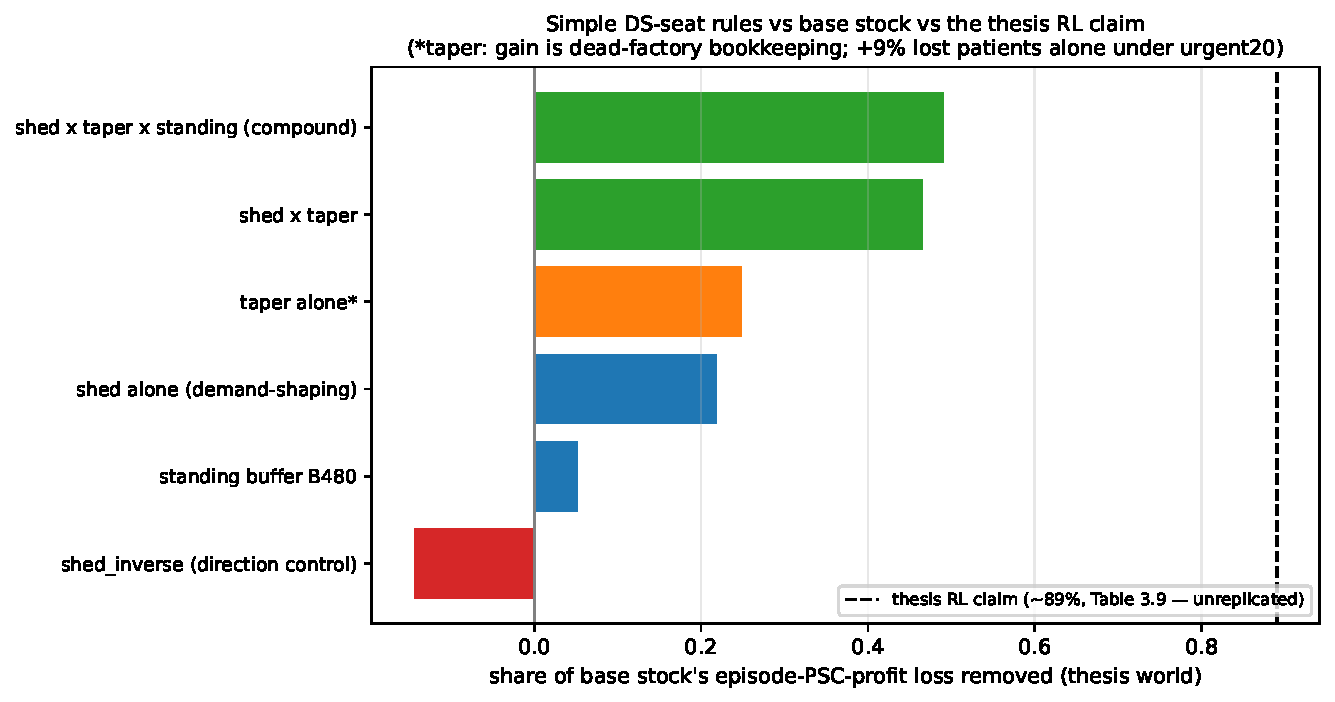
\includegraphics[width=0.92\textwidth]{../results/figures/ds_seat_shares.pdf}
\caption{Share of base stock's episode-PSC-profit loss removed by simple distributor rules
(thesis world, reporting seeds, audited). The compound reaches 49.1\% (50.7\% under urgent
demand) with fill 0.858 vs.\ 0.808 and lost patients 1,575 vs.\ 1,768. The direction
control (serve the trust-sensitive HC instead of the captive) is \emph{worse than doing
nothing} ($-$14.3\%) --- demand-shaping through the trust loop is real and directional.
State-elevated ordering is absent because it is dead by supply physics: inventory cannot
climb during the disruption (4 units measured); only the standing form pre-positions.}
\end{figure}

Reading: \textbf{simple distributor rules beat base stock decisively but reach only half of
the thesis RL's claimed 89\%}. The gap is attributable to (a) a mechanism outside the
enumerated family --- none identified --- and/or (b) baseline non-comparability: Table 3.9
is unreplicated (our own corrected-pipeline DRL run \emph{lost} to base stock), and its
exact baseline configuration is the single most valuable piece of missing information
(request pending with the thesis author). One caveat travels with the compound: the taper's
contribution is dead-factory bookkeeping under the cost lens and costs $+$9\% lost patients
\emph{when used alone} under urgent demand; the shed component offsets it.

\section{Scarcity: the frontier, the robust knob, and two honest negatives}

\begin{figure}[h]
\centering
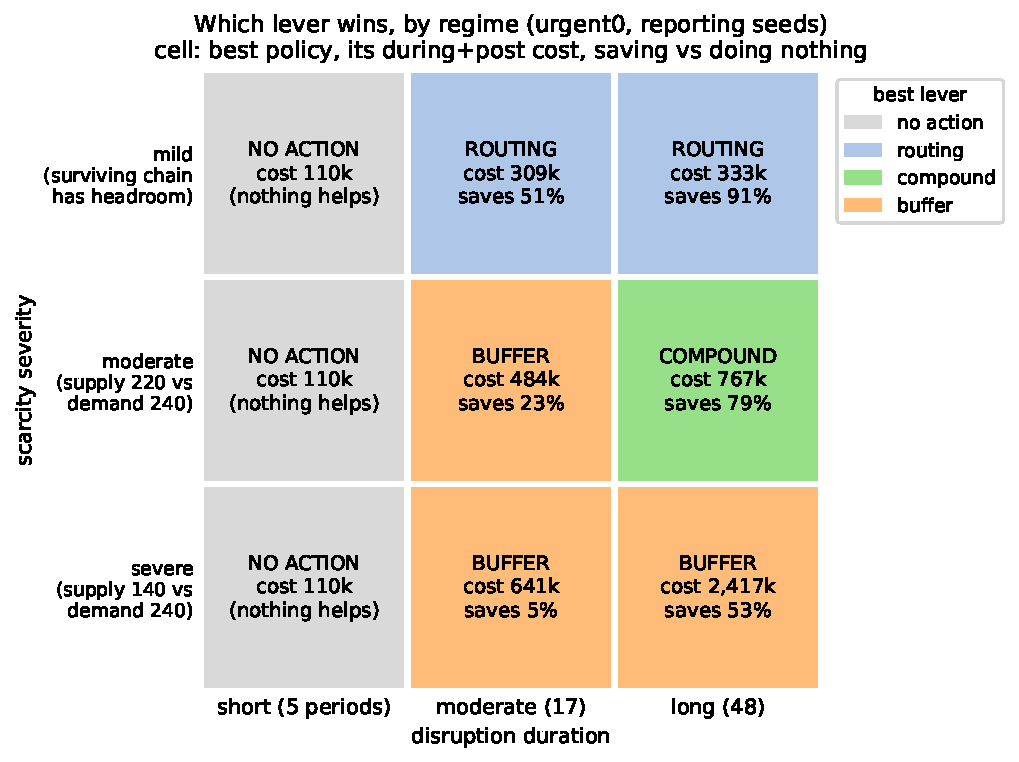
\includegraphics[width=0.74\textwidth]{../results/figures/lever_flip_map.pdf}
\caption{The lever-flip map (urgent0, reporting seeds), with the sat30/d48 cell CORRECTED
by the location screen: at severe scarcity the buffer belongs AT THE DISRUPTED CHAIN
(2,417k, $-$30\% vs.\ the healthy location) --- stock goes where the unservable demand is,
once the surviving chain is too weak to absorb rerouting. The two boundaries stand: no
response pays below the $\sim$6-period stock-cover duration; routing dominates with
surviving headroom; the compound owns mild scarcity; inventory owns severe scarcity.}
\end{figure}

\textbf{The robust knob is demand-aware buffer sizing} (B $=$ (measured demand $-$
surviving deliverable) $\times$ duration): at sat50 under urgent demand it cuts lost
patients to \textbf{41 vs.\ 505} at the frozen-grid optimum (dp-cost 1,726k vs.\ 1,865k,
reporting seeds); its other endpoint (sat30 $\to$ B=4,800) independently matched the
measured optimum.

\textbf{Negative result, kept honest:} the severity-aware redirect (cap rerouted volume at
the surviving chain's headroom) fails in BOTH natural implementations --- delivery-observation
caps throttle the supplier's ramp (orders are the production signal in this simulator), and
capacity-signal caps still under-order because over-ordering costs the orderer nothing here.
The sat30 routing penalty is a delivery-mix problem, not an order-volume problem, and is
fixed by buffer placement, not by order caps. ``One robust routing policy across the map''
does not exist in this class; per protocol the 9-cell sweep for the refuted policy was not
run.

\section{What we learned}
\begin{enumerate}
\item The decomposition: \textbf{information sharing} (largest single item at thesis
severity; two-line rule = oracle) $+$ \textbf{routing} (dominant with surviving headroom)
$+$ \textbf{inventory, correctly LOCATED and demand-SIZED} (necessary under scarcity;
location flips to the disrupted chain when the surviving chain is weak) $+$ \textbf{true
foresight} ($\sim$5\%, corrected from ``nothing'') $-$ \textbf{over-reaction} (responses
below stock-cover duration; sharp or capped rerouting under severe scarcity; clever
reactive allocation outside the captive-shed case).
\item From the DS seat, \textbf{the user's hypothesis holds in spirit}: 3 parameters of
simple rules beat base stock by half of what the RL claimed, with the residual unresolvable
until the thesis baseline is known.
\item Cleverness keeps losing to structure: five reactive rules backfired; both redirect
caps backfired; the two levers that worked everywhere are \emph{where you put stock} and
\emph{what signal you share}.
\item Process: two contaminated batches were caught by gates/diagnostics and discarded;
one rounding over-claim was caught by independent audit and corrected --- the verification
protocol earned its cost.
\end{enumerate}

\section{Next steps}
\begin{enumerate}
\item \textbf{Obtain the thesis Table 3.9 configuration} (baseline included) --- gates the
interpretation of the 49\%-vs-89\% gap; everything else about the DS-seat story is settled.
\item \textbf{Recurring-disruption axis} (held, new regime): required pre-publication
robustness check --- premium amortization could move the map's buffer cells.
\item \textbf{Ramped onset} (held): the second paper --- the one regime where detection
(vs.\ info-sharing) could earn value, given the masking result.
\item \textbf{When the corrected DRL arrives}: regime-dependent bars, all simple ---
thesis world: the DS-seat compound ($-$49\%); slack system: 273k; sat50: 767k--1,726k with
demand-aware B. Framing: measure how close learning comes to the structured optimum.
\item Paper assembly: the three-lever decomposition with the lever-flip map and the DS-seat
result as the RL-relevant centerpiece, all claims carrying their audit trail.
\end{enumerate}

\end{document}
